\chapter{\textbf{Аналитический раздел}}
\hfill

Целью работы является создание микросервиса для универсального корпоративного мессенджера. В данном разделе рассматриваются существующие решения, производится выбор СУБД. 

\section{\textbf{Постановка задачи}}

Требуется разработать микросервис универсального корпоративного мессенджера, который обладает следующей функциональностью:
\begin{itemize}
\item создание, удаление, изменение параметров пользователей, хранение истории изменений;
\item создание, удаление, изменение параметров чата, хранение истории изменений;
\item добавление, удаление, изменение параметров участников чата, хранение истории изменений;
\item отправка сообщений, файлов, хранение истории изменений;
\item возможность добавления сообщения в избранное, закрепление сообщений в чатах, хранение истории изменений. 
\end{itemize}

Система должна иметь интерфейс для демонстрации работы микросервиса. Микросервис осуществляет работу с базой данных, обрабатывает и обслуживает запросы пользователей. 

\section{\textbf{Обзор и анализ существующих решений, обоснование необходимости разработки}}

В настоящее время существует большое число различных корпоративных мессенджеров, которые решают вопрос коммуникации сотрудников внутри компании, а также поддерживает связь с клиентами, подрядчиками и партнерами  \cite{comandmessenger}.

\subsection{\textbf{Slack}}

Slack \cite{slack} -- первый корпоративный мессенджер, предложил решение, позволяющее избавиться от многочисленных писем в почте и структуризировать коммуникацию внутри команды. Далее разбивается на отдельные каналы по проектам или отделам. Имеет огромный функционал. 

В бесплатной версии Slack поддерживает неограниченное число пользователей, интеграцию с 10 внешними сервисами и поиск в архиве до 10 тысяч сообщений. В платных тарифах -- 6,67\$ (Standard) и 12,5\$ (Plus) за пользователя в месяц -- снимаются ограничения и появляются дополнительные возможности для управления правами доступа. 

На рисунке \ref{img:slack} показан интерфейс мессенджера Slack. 

\begin{figure}[H]
	\centering
	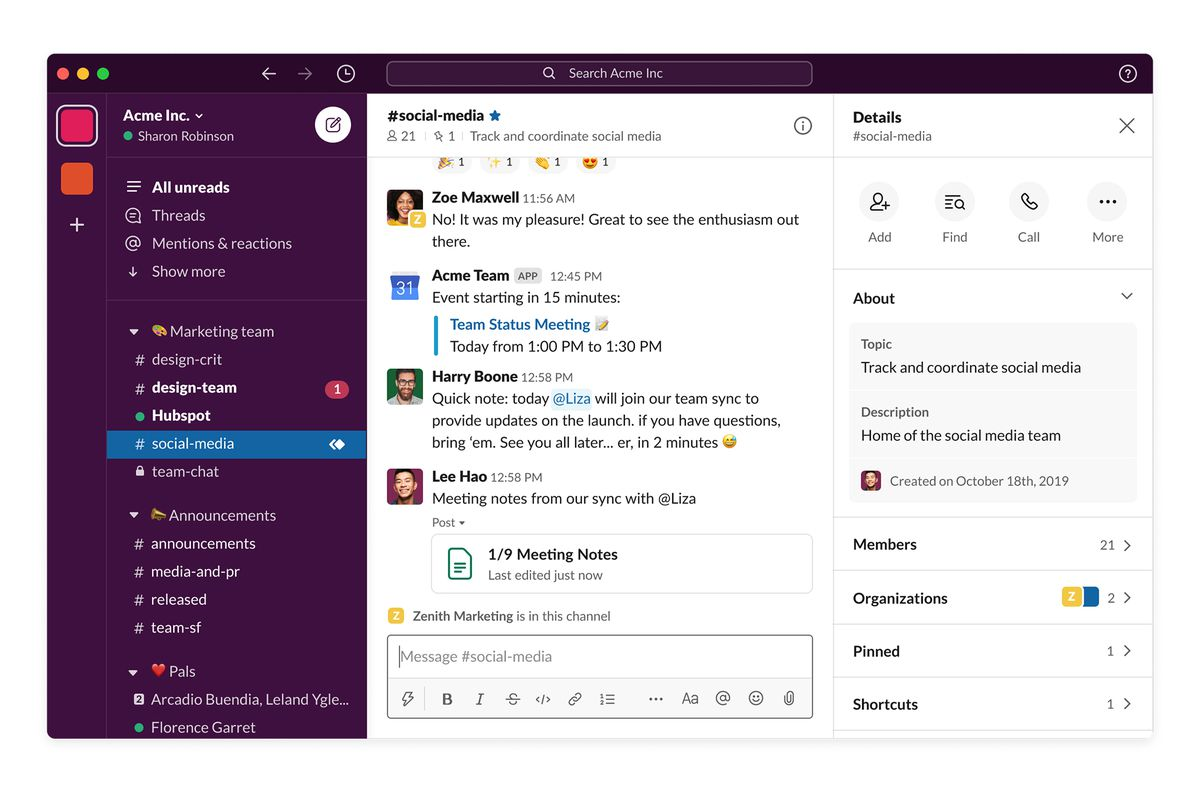
\includegraphics[scale=0.4]{slack}
	\caption{Интерфейс Slack. }
	\label{img:slack}
\end{figure}

\subsection{\textbf{Microsoft Teams}}

Microsoft Teams \cite{micteams} является альтернативой Slack. Возможность создания команд, общения посредством чата. Удобная интеграция со всеми сервисами Office 365. Однако, по сравнению со Slack, всего около 200 внешних сервисов (в Slack порядка тысячи). 

Ценовая политика лояльнее. Так, в бесплатный план входит неограниченная история сообщений, конференции до 250 человек, совместное использование экрана. Самый доступный платный план для Microsoft Teams -- \$ 5 с пользователя в месяц. 

На рисунке \ref{img:microsoftteams} показан интерфейс мессенджера Microsoft Teams. 

\begin{figure}[H]
	\centering
	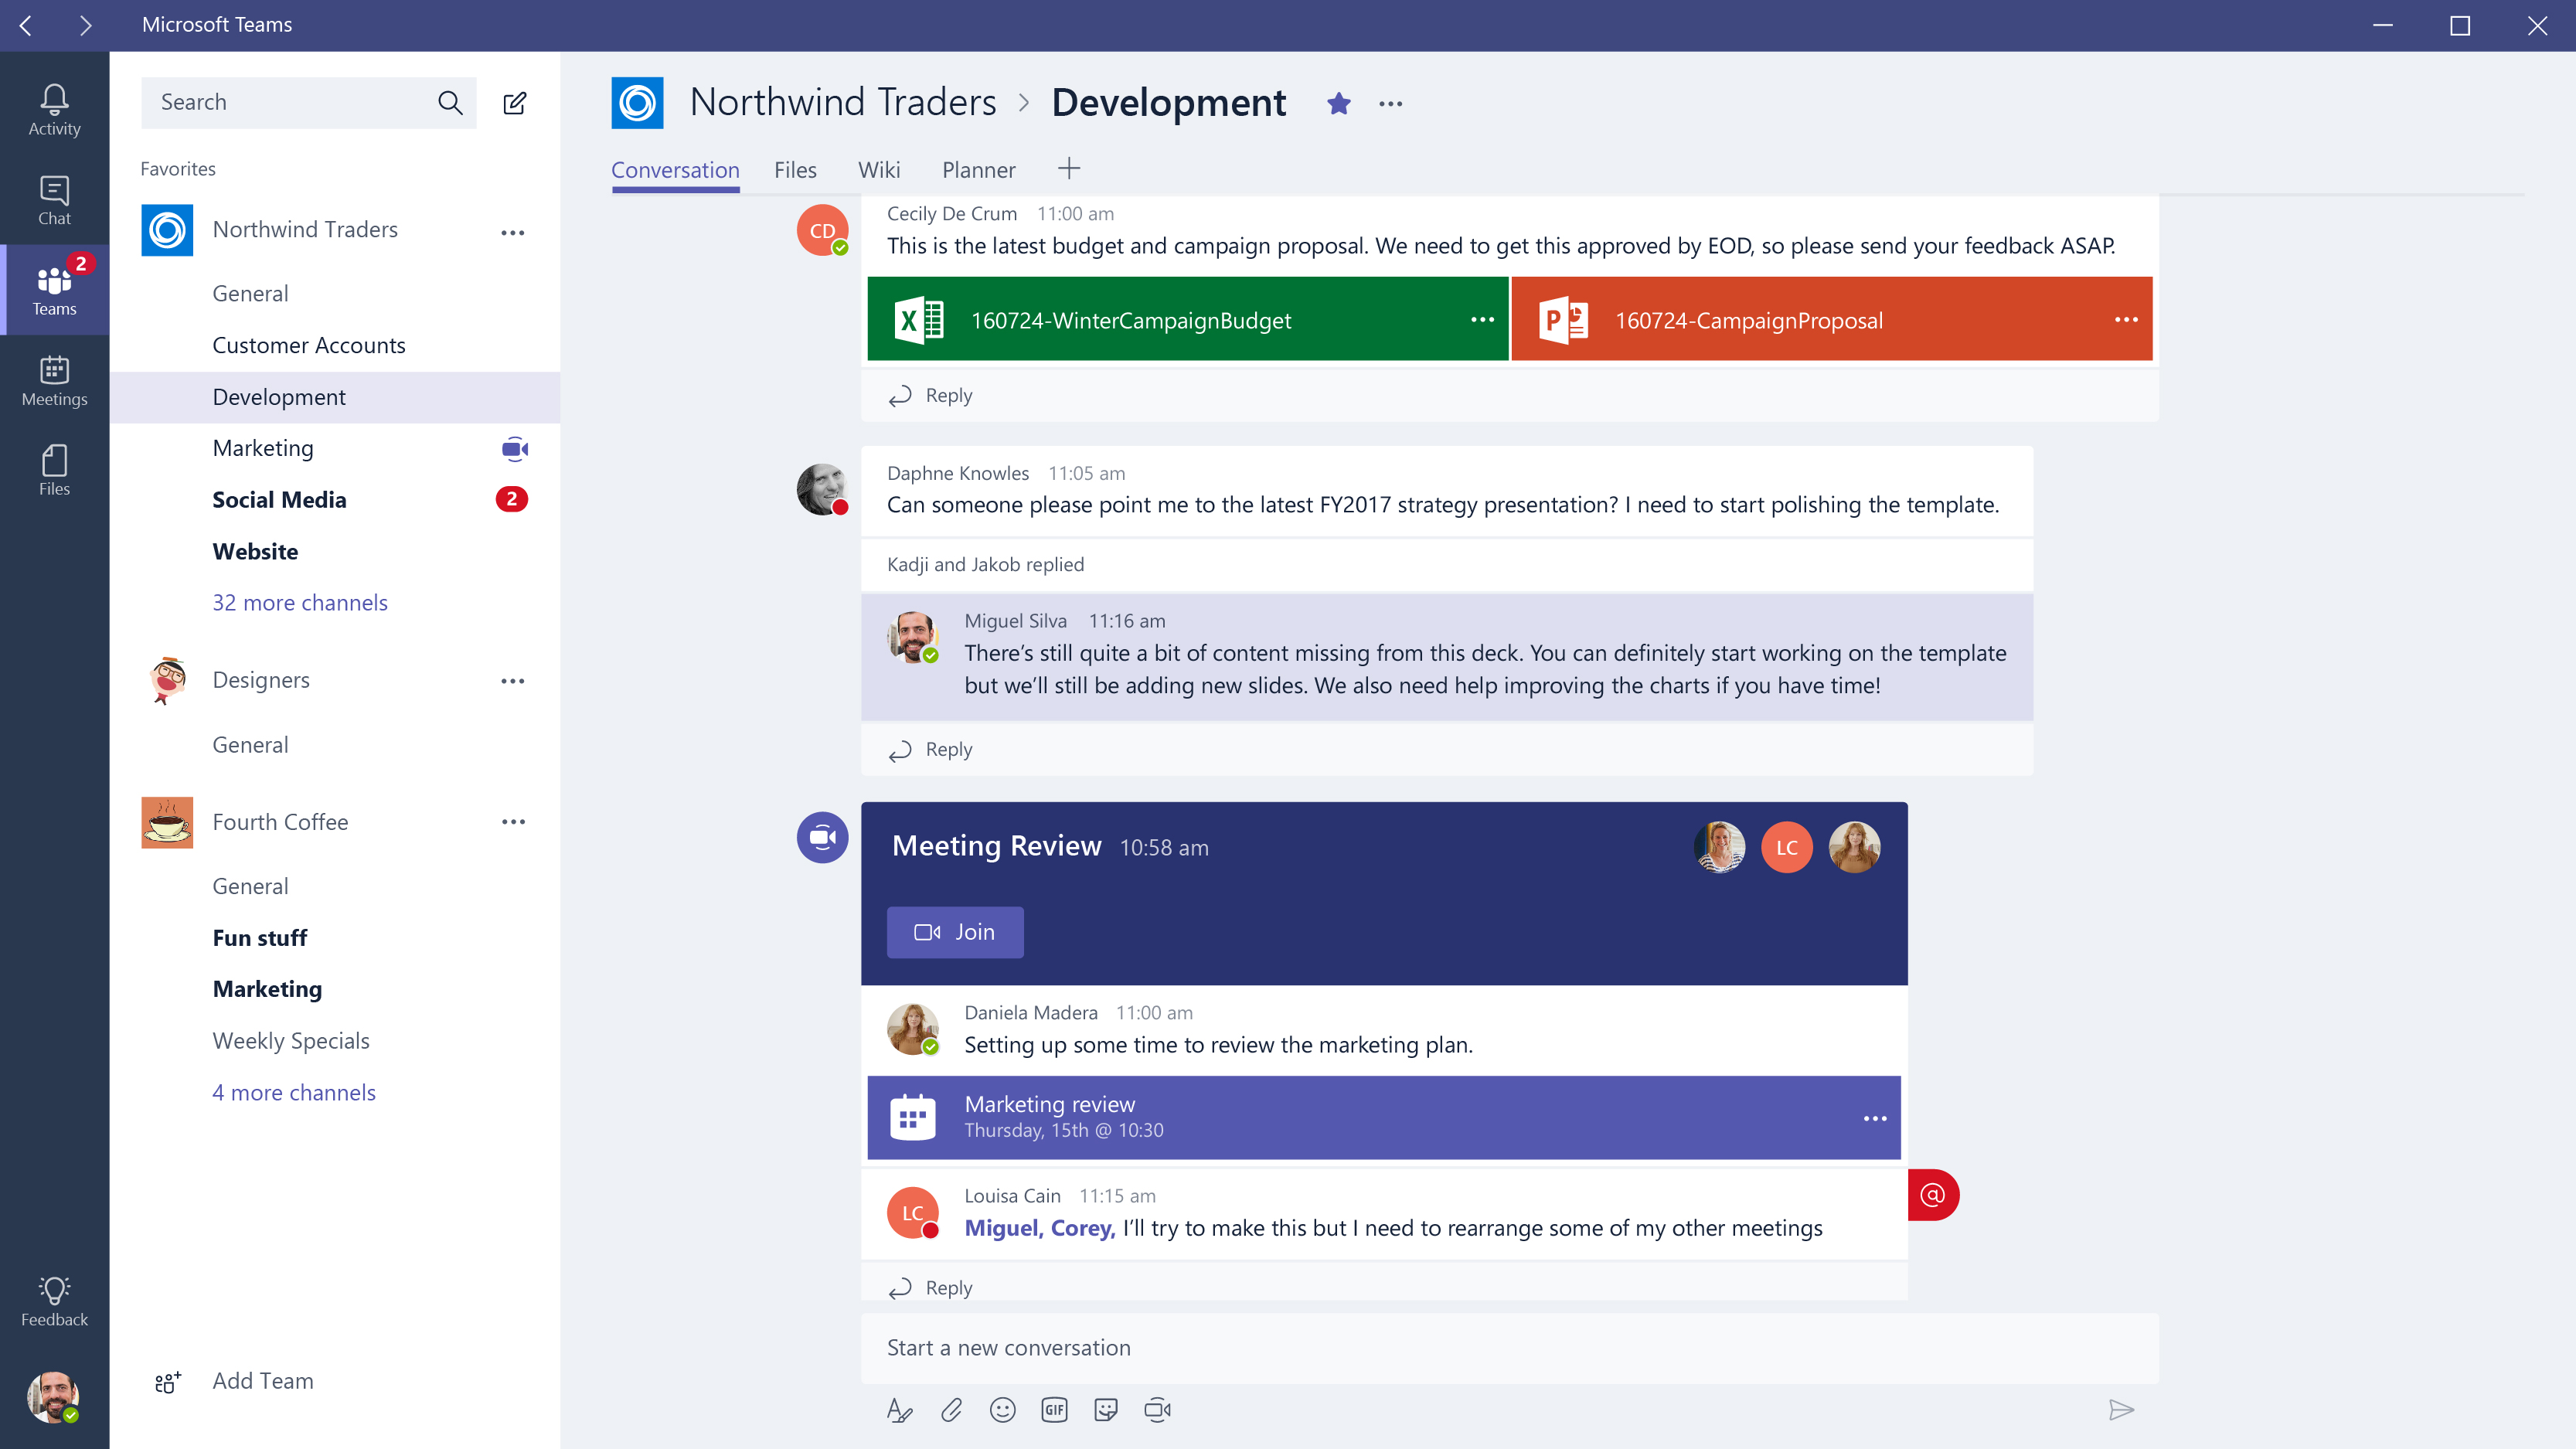
\includegraphics[scale=0.3]{microsoftteams}
	\caption{Интерфейс Microsoft Teams. }
	\label{img:microsoftteams}
\end{figure}

\subsection{\textbf{Twist}}

Twist \cite{twist} -- это успешная альтернатива Slack. Основное отличие в том, чтобы больше времени работать, и меньше отвлекаться на постоянные уведомления и чаты. Работа в мессенджере построена по принципу обсуждений -- для каждой задачи создаётся отдельный чат, в который можно пригласить членов команды. Обсуждения можно разделить по каналам -- в соответствии с общей темой. Таким образом, нет необходимости долго искать нужное обсуждение. 

Как и Slack, использование мессенджера бесплатно для команд, которым не нужен доступ к полной истории сообщений. Для остальных стоимость составит 329 $\rouble$ в месяц за человека.

На рисунке \ref{img:twist} показан интерфейс мессенджера Twist. 

\begin{figure}[H]
	\centering
	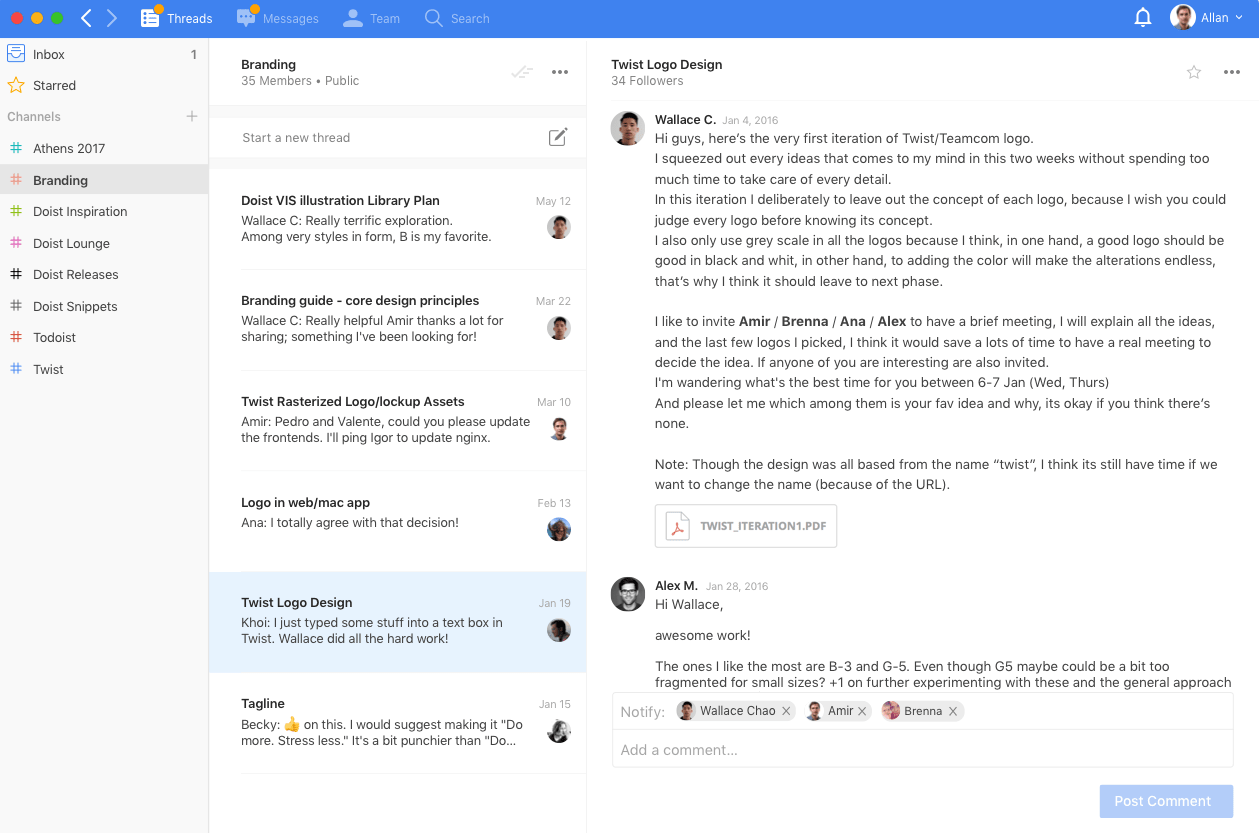
\includegraphics[scale=0.35]{twist}
	\caption{Интерфейс Twist. }
	\label{img:twist}
\end{figure}

\subsection{\textbf{Discord}}

Discord \cite{discord} -- игровой мессенджер. У пользователя в нём есть свой аккаунт, через который он может общаться с друзьями из списка контактов, а может присоединится к неограниченному количеству команд. Команды создаются бесплатно и в них также может быть неограниченное количество участников. Внутри всё устроено наподобие Slack: есть каналы, есть приватные каналы, есть возможность общаться напрямую. 

На рисунке \ref{img:discord} показан интерфейс мессенджера Discord. 

\begin{figure}[H]
	\centering
	\includegraphics[scale=0.4]{discord}
	\caption{Интерфейс Discord. }
	\label{img:discord}
\end{figure}

\subsection{\textbf{Rocket.Chat}}

Rocket.Chat \cite{rocket} --- это мессенджер с открытым исходным кодом, который поддерживает групповые чаты, обмен файлами, видеоконференции, ботов и многое другое. Rocket.Chat можно также установить на собственный сервер, а затем общаться, используя веб-интерфейс, персональный компьютер или мобильное устройство. Или использовать платную версию для облачного хранения. 

Можно добавлять новую функциональность. 

На рисунке \ref{img:rocket} показан интерфейс мессенджера Rocket.Chat. 

\begin{figure}[H]
	\centering
	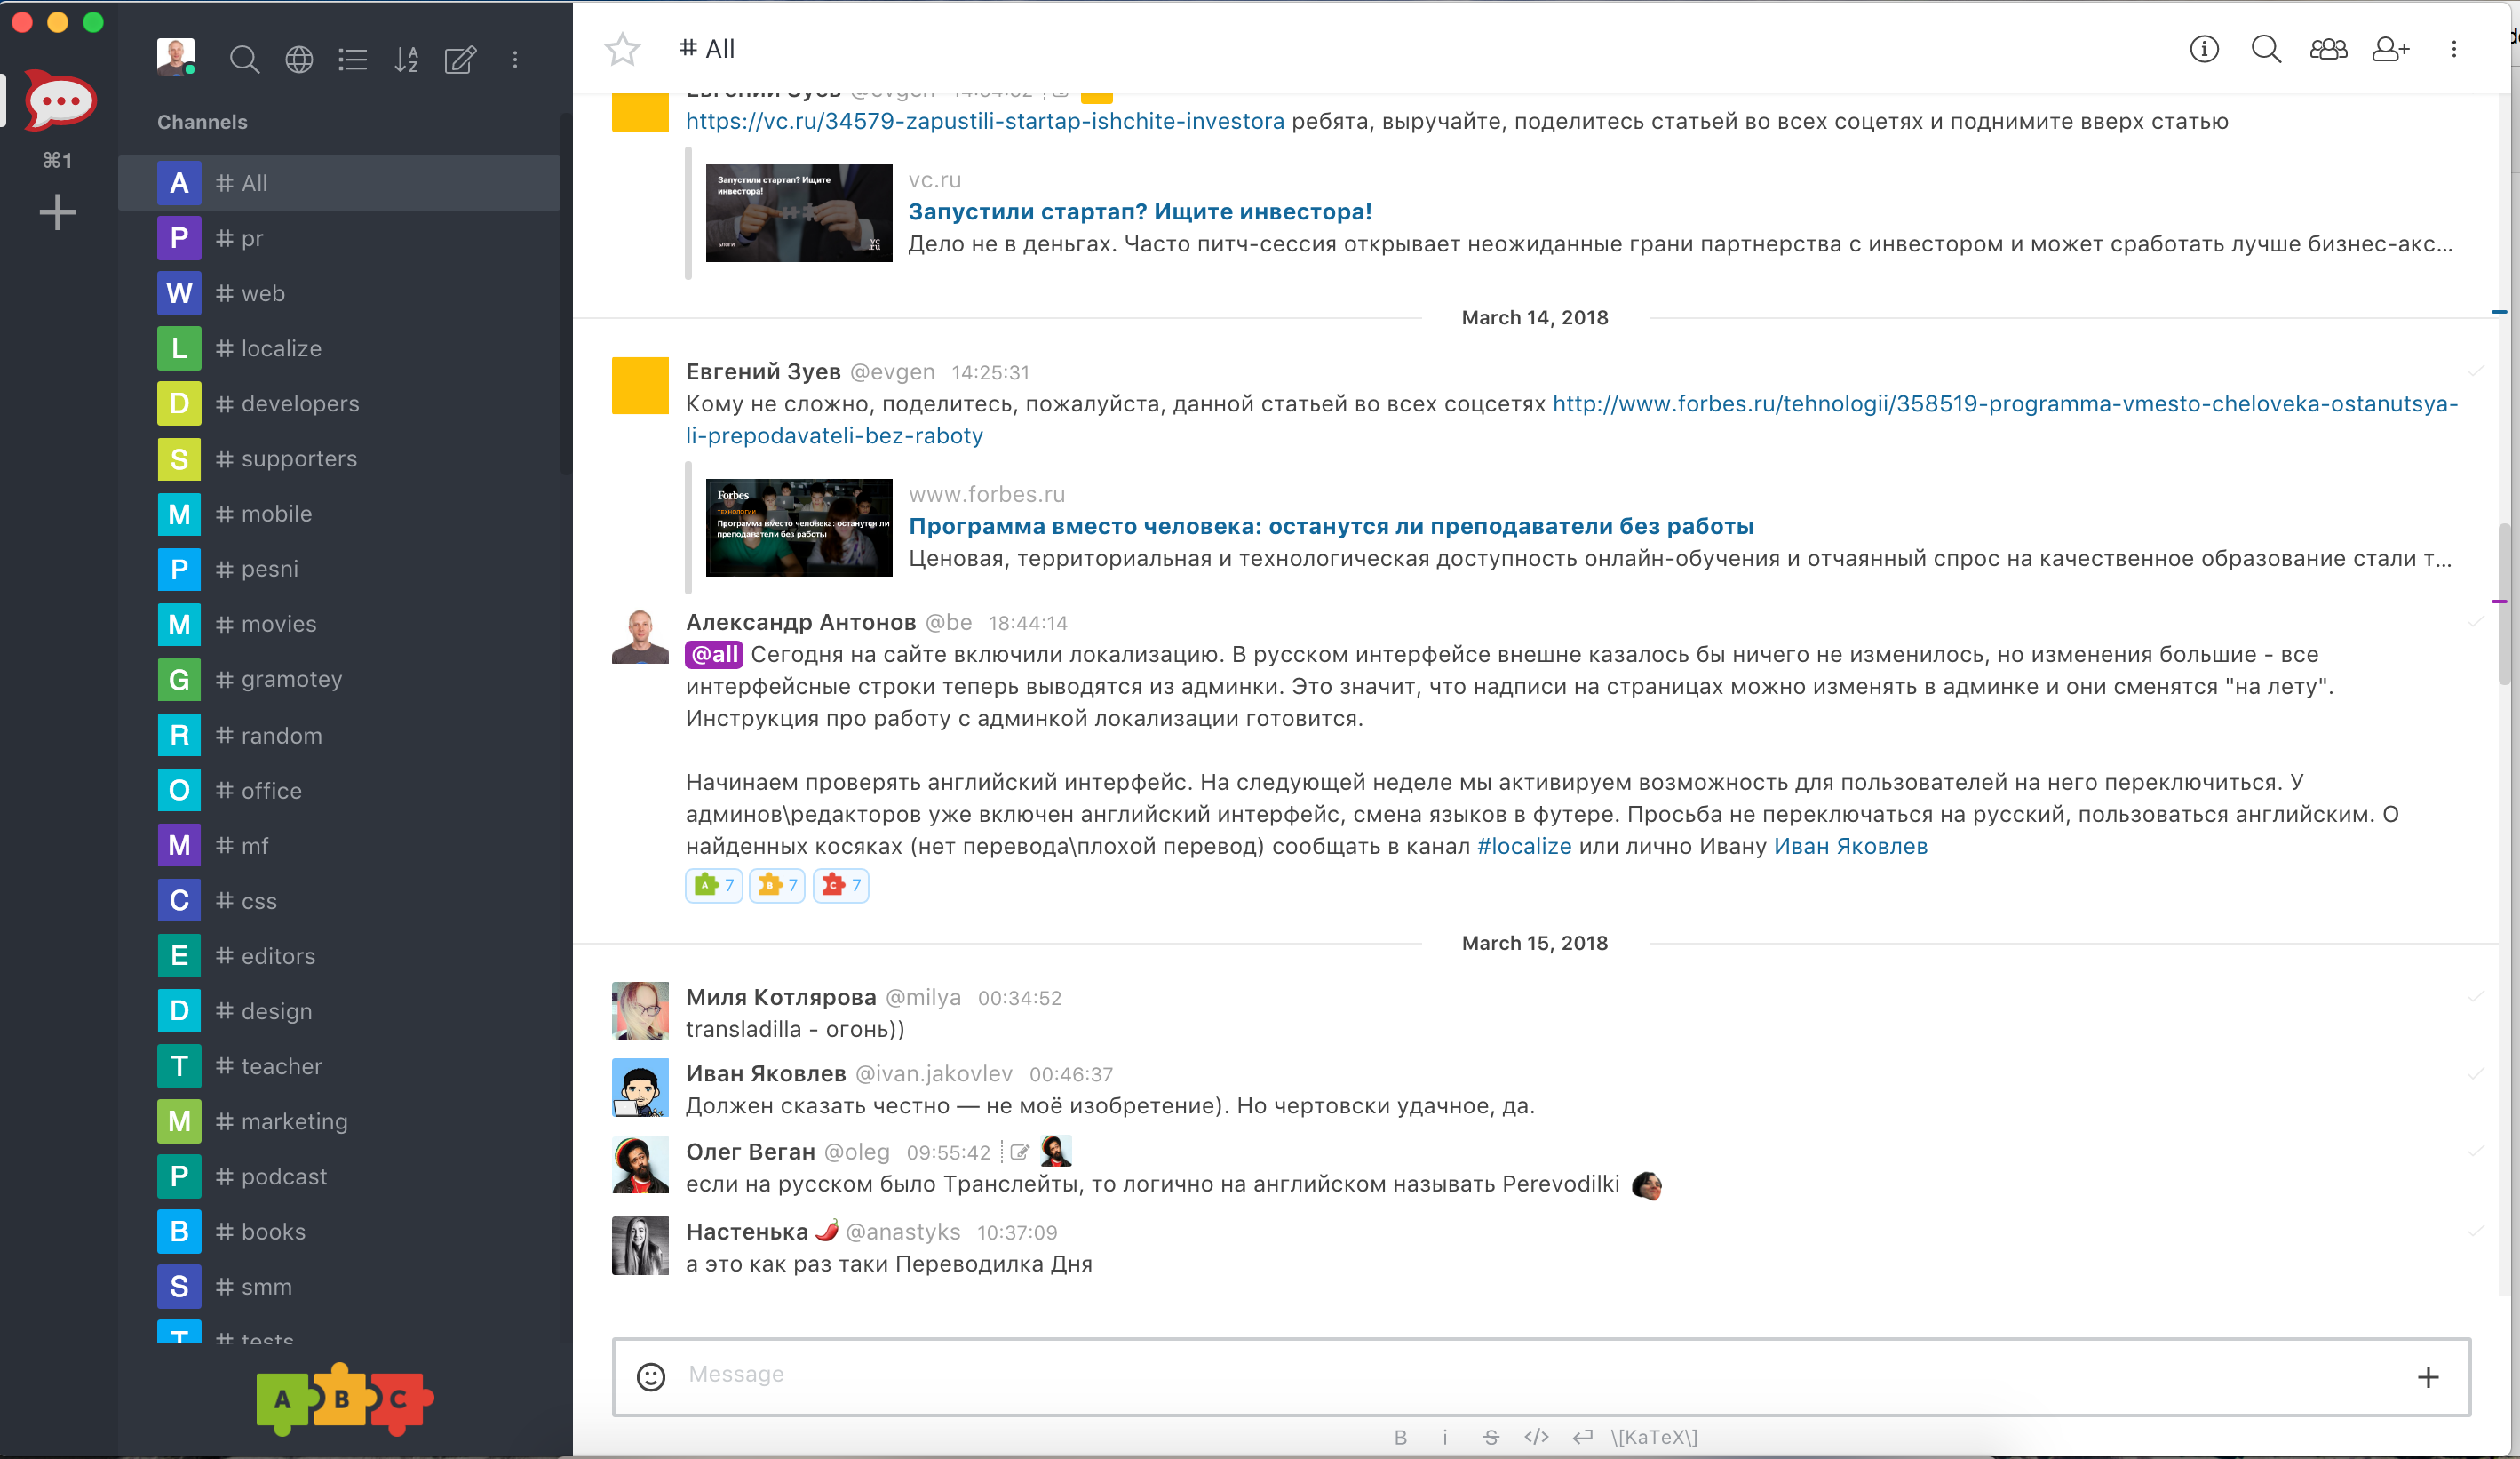
\includegraphics[scale=0.17]{rocket}
	\caption{Интерфейс Rocket.Chat. }
	\label{img:rocket}
\end{figure}


На основе аналогов и поставленных цели и задач можно выделить следующие критерии сравнения:

\begin{itemize}
\item создание обсуждения задач;
\item несколько закрепленных сообщения;
\item избранные сообщения для отдельных пользователей;
\item хранение всей истории изменений (чаты, сообщения, пользователи);
\item разные имена пользователей в различных чатах;
\item наличие различных прав у пользователей; 
\item возможность хранения на собственном сервере. 
\end{itemize}

В таблице \ref{table:messagecompare} представлено сравнение мессенджеров по вышепредставленным параметрам. 

\begin{table}[H]
\caption{Сравнение мессенджеров. }
\begin{tabular}{|p{5cm}|p{1.9cm}|p{1.9cm}|p{1.9cm}|p{1.9cm}|p{1.5cm}|}
\hline
 & Slack & Microsoft Teams  & Twist & Discord & Rocket. Chat  \\ \hline
Создание обсуждения задач & + (прям в чате) & + & + & - & - \\ \hline
Несколько закрепленных сообщения & +  & - & - &  + (ограничение 50)  & +  \\ \hline
Избранные сообщения для отдельных пользователей  & +  & - & - & -  & + \\ \hline
Хранение всей истории изменений (чаты, сообщения, пользователи)& - &-& - & - & - \\ \hline
Разные имена пользователей в различных чатах& - & +& - &  + & + \\ \hline
Наличие различных прав у пользователей& - & + & + &  + & + \\ \hline
Возможность хранения на собственном сервере& - & - & - &  - & + \\ \hline
\end{tabular}
\label{table:messagecompare}
\end{table}

\textbf{Актуальность темы} обусловлена отсутствием универсального мессенджера с полной историей изменения чатов, пользователей, сообщений. А ещё у рассмотренных готовых решений вся переписка хранится на облачных серверах мессенджера. Данный факт не устраивает большое количество компаний, которым желательно хранить все данные на своих серверах. 

\section{\textbf{Анализ типов и выбор СУБД}}

Цели и задачи поставлены необходимо определиться с СУБД. 

\subsection{\textbf{Типы СУБД}}

Системы управления базами данных (СУБД) -- это высокоуровневое программное обеспечение, работающее с низкоуровневыми API. Для решения проблем создавались различные виды СУБД. Два основных направления -- реляционные (SQL) и нереляционные (NoSQL) СУБД \cite{nosql}. СУБД основаны на моделях баз данных. 

\subsubsection{\textbf{Реляционная модель}}

Представленная в 70-х, реляционная модель предлагает структурированное хранение данных. Отношения дают возможность группировки данных как связанных наборов, представленных в виде таблиц, содержащих упорядоченную информацию и соотносящих значения и атрибуты. РСУБД работают производительно и надёжно. Несмотря на строгие принципы формирования и обработки данных, РСУБД могут быть гибкими.

\subsubsection{\textbf{Иные подходы}}

NoSQL-способ структуризации данных заключается в избавлении от ограничений при хранении и использовании информации. Базы данных NoSQL, используя неструктуризированный подход, предлагают много эффективных способов обработки данных в отдельных случаях. 

В таблице \ref{table:subd} представлено сравнение 2 этих подходов. 

\begin{table}[H]
\caption{Сравнение моделей БД. }
\begin{tabular}{|p{5cm}|p{5cm}|p{5cm}|}
\hline
 & SQL & NoSQL  \\ \hline
Структура и тип хранящихся данных & Однозначно определёная структура хранения данных & Ограничений нет \\ \hline
Запросы & Получение данных при помощи языка SQL&  Каждая NoSQL база данных реализует свой способ работы с данными \\ \hline
Масштабируемость  & Не подходит для постоянно меняющихся структур данных & Подходит для постоянно меняющихся структур данных \\ \hline
Поддержка & Развитая СУБД, наличие большого сообщества вокруг неё, множество примеров & Только недавно стала популярной \\ \hline
Объединение таблиц & Применени join & Отсутствие join \\ \hline
\end{tabular}
\label{table:subd}
\end{table}

Так как, данные имеют четкую структуру и заранее определены, выбор в пользу реляционной базы данных. 

\subsection{\textbf{Выбор реляционной СУБД}}

Одними из самых популярных РСУБД сейчас являются MSSQL, MySQL, PostgreSQL, Oracle.

\subsubsection{\textbf{MSSQL}}

Microsoft SQL Server -- разработанная корпорацией майкрософт, система управления реляционными базами данных.

Преимущества
\begin{itemize}
\item простота: MSSQL легко устанавливается и используется;
\item возможность регулировки и отслеживания уровня производительности, чтобы уменьшить загрузку;
\item возможность интеграции с другими продуктами Microsoft;
\item визуализация на мобильных устройствах.
\end{itemize}

Недостатки
\begin{itemize}
\item высокая стоимость продукта для юридических лиц;
\item возможны проблемы в работе служб интеграции импорта файлов;
\item высокая ресурсоемкость SQL Server.
\end{itemize}

\subsubsection{\textbf{MySQL}}

MySQL -- это самая популярная из всех крупных серверных БД. Разобраться в ней просто, большое количество информации. 

Преимущества
\begin{itemize}
\item простота: MySQL легко устанавливается и используется;
\item много функций: MySQL поддерживает большую часть функционала SQL;
\item безопасность: в MySQL встроено много функций безопасности;
\item мощность и масштабируемость: MySQL может работать с действительно большими объёмами данных, и неплохо походит для масштабируемых приложений;
\item скорость: пренебрежение некоторыми стандартами позволяет MySQL работать производительнее.
\end{itemize}

Недостатки
\begin{itemize}
\item ограничения функциональности, так как не полностью реализованы SQL-стандарты;
\item надёжность: некоторые операции реализованы менее надёжно, чем в других РСУБД;
\item застой в разработке: хотя MySQL и является open-source продуктом, работа над ней сильно заторможена.
\end{itemize}

\subsubsection{\textbf{PostgreSQL}}

PostgreSQL -- это РСУБД, ориентирующаяся в первую очередь на полное соответствие стандартам и расширяемость.

Преимущества
\begin{itemize}
\item полная SQL-совместимость;
\item cообщество: PostgreSQL поддерживается опытным сообществом 24/7;
\item поддержка сторонними организациями;
\item расширяемость: PostgreSQL можно программно расширить за счёт хранимых процедур. 
\end{itemize}

Недостатки
\begin{itemize}
\item производительность: в простых операциях чтения PostgreSQL может уступать своим аналогам. 
\end{itemize}

\subsubsection{\textbf{Oracle}}

Oracle -- это объектно-реляционная система управления базами данных.

Преимущества
\begin{itemize}
\item поддержка огромных баз данных и большого числа пользователей;
\item быстрая обработка транзакций;
\item большой и постоянно развивающийся функционал. 
\end{itemize}

Недостатки
\begin{itemize}
\item высокая стоимость;
\item требуются значительные вычислительные ресурсы.  
\end{itemize}

PostgreSQL выигрывает по многим параметрам и бесплатно распространяется. Поэтому было принято решение использовать именно эту РСУБД.

\section{\textbf{Вывод}}

В данном разделе были рассмотрены существующие решения, была выбрана СУБД и поставлена задача реализации микросервиса мессенджера с хранением истории, возможностью добавлять сообщения в избранное и закреплять в чатах. 